\chapter{Kravspecifikationer}

\section{Optimale løsningsforslag}
Den ideelle løsning vil bestå af to dele, en mobiltelefon med GPS og en website/server som kan vise dataene sendt fra mobilen

Mobilen skal kunne:
\begin{itemize}
	\item Måle, sende og optage GPS positionen på løberen undervejs på ruten.
	\item Tilslutte sig en bestemt bane, som træneren har opsat og lagt på serveren inden træning.
	\item Mobilen må ikke hjælpe løberen undervejs i løbet, med at vise positionen på ruten.
\end{itemize}

Websitet/serveren skal kunne:
\begin{itemize}
	\item Opsætte baner inden løbet.
	\item Vise løbernes position på kortet.
	\item Vise diverse statistik og data for løberens tur på banen. Dette vil være tider, afstande og hastigheder, samt en grafisk visning af den rute løberen har løbet.
	\item Sammenligne to løberes tur på samme rute, eller sammenligne med banens gennemsnit i forhold til statistik/rådata.
	\item Vise et grafisk replay af den rute løberen har løbet, med mulighed for at afspille flere løbere samtidig og dermed sammenligne vejvalg.
	\item Være kompatibelt med GPS-ure.
\end{itemize} 

Mobil-appen vil have en simpel brugergrænseflade hvor brugeren vil have mulighed for at vælge den bane vedkommende skal løbe. Herefter vil brugeren have mulighed for at trykke start, hvorefter mobilen kun vil vise hvor lang tid der er brugt indtil videre og en afslut knap. Under løbet sender mobilen løbende data om GPS position og tiden siden start. Når turen er løbet færdig trykker brugere på afslut og appen vil sende de sidste data og vise nogle resultater. Dette kan eksempelvis være tid i alt, højeste hastighed, gennemsnitshastighed, men også data om løberen sammenlignet med andre på samme bane. Dette kan f. eks. være hvor mange sekunder efter den hurtigste vedkommende har brugt på de enkelte stræk.

Inden løbet skal træneren eller arrangøren, kunne uploade den bane som personen har lavet, til serveren. Banerne kan vælges fra appen på mobilen, af de forskellige løbere. Efter løbet skal brugerne som sagt kunne uploade sine resultater til websitet/serveren fra mobil appen, under og efter et endt løb. Disse resultater skal så kunne sammenlignes med de andre løbere, der har løbet den samme bane. Ud over at sammenligne statistik over løberens rute, som beskrevet ovenfor, skal den også kunne vise grafisk den rute som løberen har løbet. Derudover skal der være en replay funktion, så de vejvalg som løberen tager, kan ses. Så kan der indsættes flere løbere på den grafiske visning, så flere løberes vejvalg kan sammenlignes.

\subsection{Krav til optimalløsning}
Ud fra overstående har gruppen opstillet noglle krav til den optimaleløsning. Som udgangspunkt har gruppen gået ud fra at kravene skal være testbare. 

\begin{itemize}
\item Appen tilknyttet løsningen skal kunne køre på android smartphones og apple iphones.
\item Løsningen skal være en webservice.
\item Samme loginsystem for både app og webservice.
\item Webservicen skal kunne oprette og gemme baner i form af o-løbskort med integnede poster.
\item Webservicen skal grafisk kunne vise en eller flere GPS ruter uploaded fra appen ovenpå den tilknyttede bane (Kort)
\item webservicen skal have følgende replay funktionaliteter:
\begin{itemize}
\item Det skal være muligt at til/fravælge løbere til den viste bane, evt. mulighed for at tilpasse halelængde og farve
\item Zoom funktion på kortet. (senere måske rotationsfunktion så kortet kan roteres og få strækretningen op på kortet.)
\item Det skal være muligt at starte og pause afpilningen af GPS Dataene.
\item Det skal være muligt at sætte tempoet til 1, 2, 5, 10 og 20 gange normal hastighed
\item Scrolling function for at komme hurtigt frem til et bestemt tidspunkt.
\item Det skal være muligt at vælge én post (punkt som alle passerer) hvor alle viste løbere bliver samlet ved. Der skal kunne defineres/vælges flere poster/punkter
\end{itemize}
\item Webservicen skal kunne vise følgende data for hvert stræk:
\begin{itemize}
\item Den enkelte løbers navn
\item Den enkelte løbers placering i løbet efter strækket
\item Den enkelte løbers stræk længde
\item Den enkelte løbers tilbagelagte rute
\item Den enkelte løbers samlede tid efter strækket
\item Den enkelte løbers tid på strækket
\item Den enkelte løbers tid i forhold til den hurtigste på strækket
\item Den enkelte løbers gns. fart på strækket
\item Den enkelte løbers top fart på strækket
\item Evt grafisk sammenligning mellem to løbere ved at tegne streger mellem de to løberes placering på samme tid efter udgangspunktet.
\end{itemize}
\item Appen skal kunne optage gps-data under løb og ved løbets afslutning sende disse til webserveren.
\item Appen skal kunne tilknytte sig en bane, oprettet på webservicen.
\item Appen skal kunne sortere banerne ud fra klub.
\item Appen må kun vise tid brugt hidtil og en afslutningsknap på skærmen under løbet.
\item Appen skal kunne tilgå og grafisk vise webservicens replayfunktionaliteter.
\item Appen skal være brugervenlig, i den forstand, at det skal være let at vælge en bane, starte et løb, afslutte et løb og bruge replay-funktionen. Navigering i appen skal være simpel.
\end{itemize}

\subsection{Mugshots af optimalløsning}
\subsubsection{Mobilenhed}
Gruppen har gjort sig nogle tanker om hvordan den opmitaleløsning skal se ud og hvilke funktioner den skal have. Udfra dette er der blevet lavet nogle mugshots af hvordan gruppen tæntke den optimale løsning kunne komme til at se ud.

\begin{figure}
\centering
\begin{minipage}{.5\textwidth}
  \centering
  \fbox{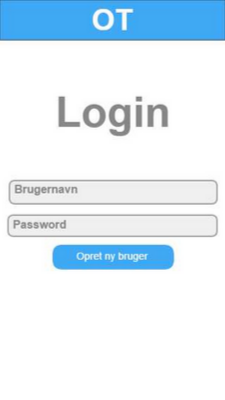
\includegraphics[width=.5\linewidth]{billeder/Mobilversion_1}}
  \caption{Almindelig skærmpost}
  \label{fig:test1}
\end{minipage}%
\begin{minipage}{.5\textwidth}
  \centering
  \fbox{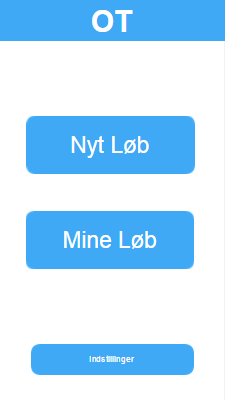
\includegraphics[width=.5\linewidth]{billeder/Mobilversion_2}}
  \caption{Elektronisk post}
  \label{fig:test2}
\end{minipage}
\end{figure}

Figur 4.1 viser det første der ses når appen åbnes på ens smartphone. Der er to muligheder på denne side, enten kan der logges ind med en eksisterende bruger, eller også kan der oprettes en ny bruger. 

Hvis det lykkes at logge ind på appen, vil det næste der ses være figur 4.2, hvor der ses tre knapper. Der er mulighed for at påbegynde et nyt løb, der kan ses på de løb brugeren allerede har løbet, eller der kan ændres i ens indstillinger.

\begin{figure}
\centering
\begin{minipage}{.5\textwidth}
  \centering
  \fbox{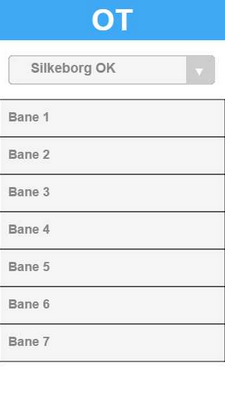
\includegraphics[width=.5\linewidth]{billeder/Mobilversion_3}}
  \caption{Almindelig skærmpost}
  \label{fig:test1}
\end{minipage}%
\begin{minipage}{.5\textwidth}
  \centering
  \fbox{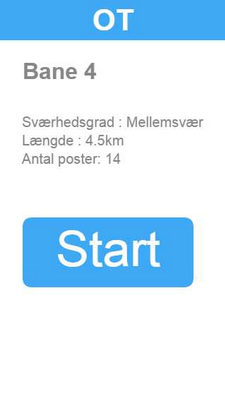
\includegraphics[width=.5\linewidth]{billeder/Mobilversion_4}}
  \caption{Elektronisk post}
  \label{fig:test2}
\end{minipage}
\end{figure}
Hvis menu punktet ”Nyt løb” vælges, bliver brugeren ført videre til figur 4.3. Øverst i appen kan der ses en dropdown menu, hvor der er mulighed for at vælge den o-løbs forening som der løbes for. Under den valgte o-løbs forening, vil der så være et antal baner brugeren kan vælge at løbe. Det er foreningen selv der skal uploade de baner som er muligt at løbe, hvor det så er planen at en forening skal have et administrator login, for at kunne uploade disse baner.

\begin{figure}
\centering
\begin{minipage}{.5\textwidth}
  \centering
  \fbox{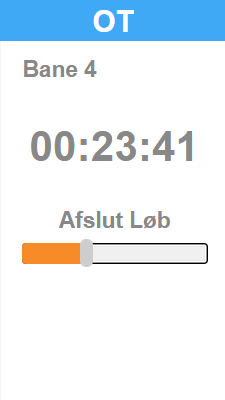
\includegraphics[width=.5\linewidth]{billeder/Mobilversion_5}}
  \caption{Almindelig skærmpost}
  \label{fig:test1}
\end{minipage}%
\begin{minipage}{.5\textwidth}
  \centering
  \fbox{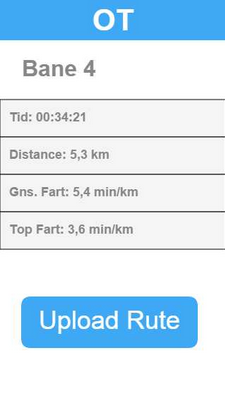
\includegraphics[width=.5\linewidth]{billeder/Mobilversion_6}}
  \caption{Elektronisk post}
  \label{fig:test2}
\end{minipage}
\end{figure}

Trykkes der på en af banerne, eksempelvis bane 4.4, føres brugeren ind på siden set på figur 4.4. Her ses nogle informationer om det valgte løb, samt en stor ”Start” knap, hvor løbet selvfølgelig startes. De informationer der findes om løbet er sværhedsgraden på banen, ca. længden på banen, samt hvor mange poster løberen skal igennem. Hvis bane 4 er den bane brugeren gerne vil løbe, trykker brugeren på ”Start” knappen. Brugeren kommer så ind på en siden vist på figur 4.5. Denne figur afbilleder hvad der kan ses underløbet. Det er ikke muligt at se noget kort, da appen ikke skal vise løberens position på kortet. Det eneste der kan ses, er hvilken bane der er valgt, den tid der er gået siden der er trykket ”Start” og en slide knap til at afslutte løbet.
\begin{figure}
\centering
\begin{minipage}{.5\textwidth}
  \centering
  \fbox{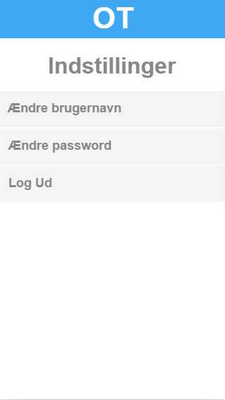
\includegraphics[width=.5\linewidth]{billeder/Mobilversion_7}}
  \caption{Almindelig skærmpost}
  \label{fig:test1}
\end{minipage}%
\begin{minipage}{.5\textwidth}
  \centering
  \fbox{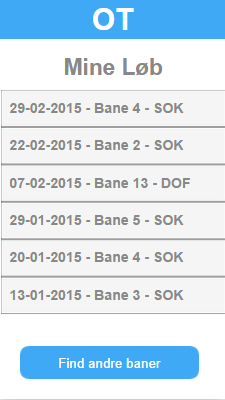
\includegraphics[width=.5\linewidth]{billeder/Mobilversion_8}}
  \caption{Elektronisk post}
  \label{fig:test2}
\end{minipage}
\end{figure}

Når løberen har været igennem alle poster og kommet i mål, bruges slide knappen ”Afslut løb”, dette fører brugeren ind på figur 4.6. Dette skal vise informationer om den netop færdiggjorte bane. Her ses tiden fra start til slut, den distance løberen har løbet, gennemsnitsfart og løberens top fart. I bunden af siden ses en ”Upload Rute” knap, trykkes der på denne knap uploades ens rute, over den bane der lige er blevet løbet, til webserveren. Nu kan løberens resultater sammenlignes med andre løberes resultater, på den specifikke bane.

Kigges der igen på figur 4.2 og menupunktet ”Indstillinger” vælges, bliver brugeren ført ind til figur 4.7. Her kan brugeren ændre sit brugernavn, sit password og vælge at logge ud fra appen.

Hvis menupunktet ”Mine løb” vælges i figur 4.2, kan brugeren se en liste over sine gennemførte løb, som ses på figur 4.8. Listen er sorteret efter dato, hvor de nyeste løb vil være øverst. Derudover kan der ses hvilken bane der er blevet løbet, samt hvilken forening der er blevet løbet ved. I bunden af siden er der en ”Find andre baner” knap, hvor der kan søges efter alle de baner der findes i databasen. Derudover kan der søges efter en specifik o-løbs forening eller dato, på denne måde kan der findes løb der er blevet løb på samme bane og dag som brugeren selv har løbet som ses på figur 4.9. De fundne baner kan så bruges til at sammenlignes med brugerens egne resultater på samme bane.

\begin{figure}
\centering
\begin{minipage}{.5\textwidth}
  \centering
  \fbox{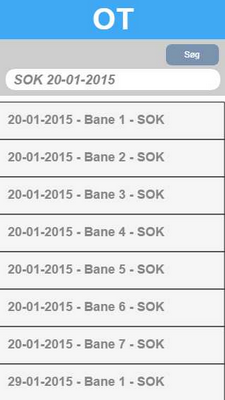
\includegraphics[width=.5\linewidth]{billeder/Mobilversion_9}}
  \caption{Almindelig skærmpost}
  \label{fig:test1}
\end{minipage}%
\begin{minipage}{.5\textwidth}
  \centering
  \fbox{\includegraphics[width=.5\linewidth]{billeder/Mobilversion_10}}
  \caption{Elektronisk post}
  \label{fig:test2}
\end{minipage}
\end{figure}

Hvis brugeren har valgt at ville sammenligne løbere på en specifik bane, vil brugeren se en side lignende figur 4.10. I toppen af siden ses tre knapper. Den første er den side der allerede ses, hvor der er en grafisk visning af løberne på deres rute. Der ses en blå, rød og grøn slange på kortet, som er løberne. Under kortet findes der nogle mediaplayer funktioner. Den første knap er play/pause, den anden knap(flaget) bruges til at vælge hvilken post der ønskes sammenlignes fra. Normalt løber løberne ikke på samme tid, det ønskes dog lavet sådan, at det er muligt at sammenligne løbere fra en bestemt post. Dette betyder hvis løber 1 har en stræk tid på 2 min på post 1 og løber 2 har en stræk tid på 25 min på post 1, hvis løberne så ønskes sammenlignet fra post 1, ses der fra deres begyndelse fra post 1, lige gyldigt hvor lang tid de har brugt tidligere. De næste to knapper i mediaplayer funktionerne, bruges til at hoppe frem og tilbage mellem poster. Den sidste knap er en reset knap, hvor den fjerner alle de ændring brugeren har lavet tidligere, og sætter det op som det var i begyndelsen.  

Andet menupunkt i toppen, indeholder forskellige informationer om løberne. Dette er deres tider, distancer osv., så løberne også kan sammenlignes med tal og ikke kun grafisk. Sidste menupunkt er en guide der skal forklare hvordan dette sammenlignings værktøj bruges. Det skal forklare hvad de forskellige funktioner gør og hvordan de bruges.

Nederst på siden ses en knap ”Løbere”. Trykkes der på denne knap, skal et nyt vindue poppe op, hvor der skal være en liste over hvilke løbere der er med, og hvilken farve de har på kortet.
\subsubsection{Webservice}
Interfaceet på webservicen ligner meget interfacet på appen fra figur 4.10. 
\begin{figure}[h]
    \centering
    \fbox{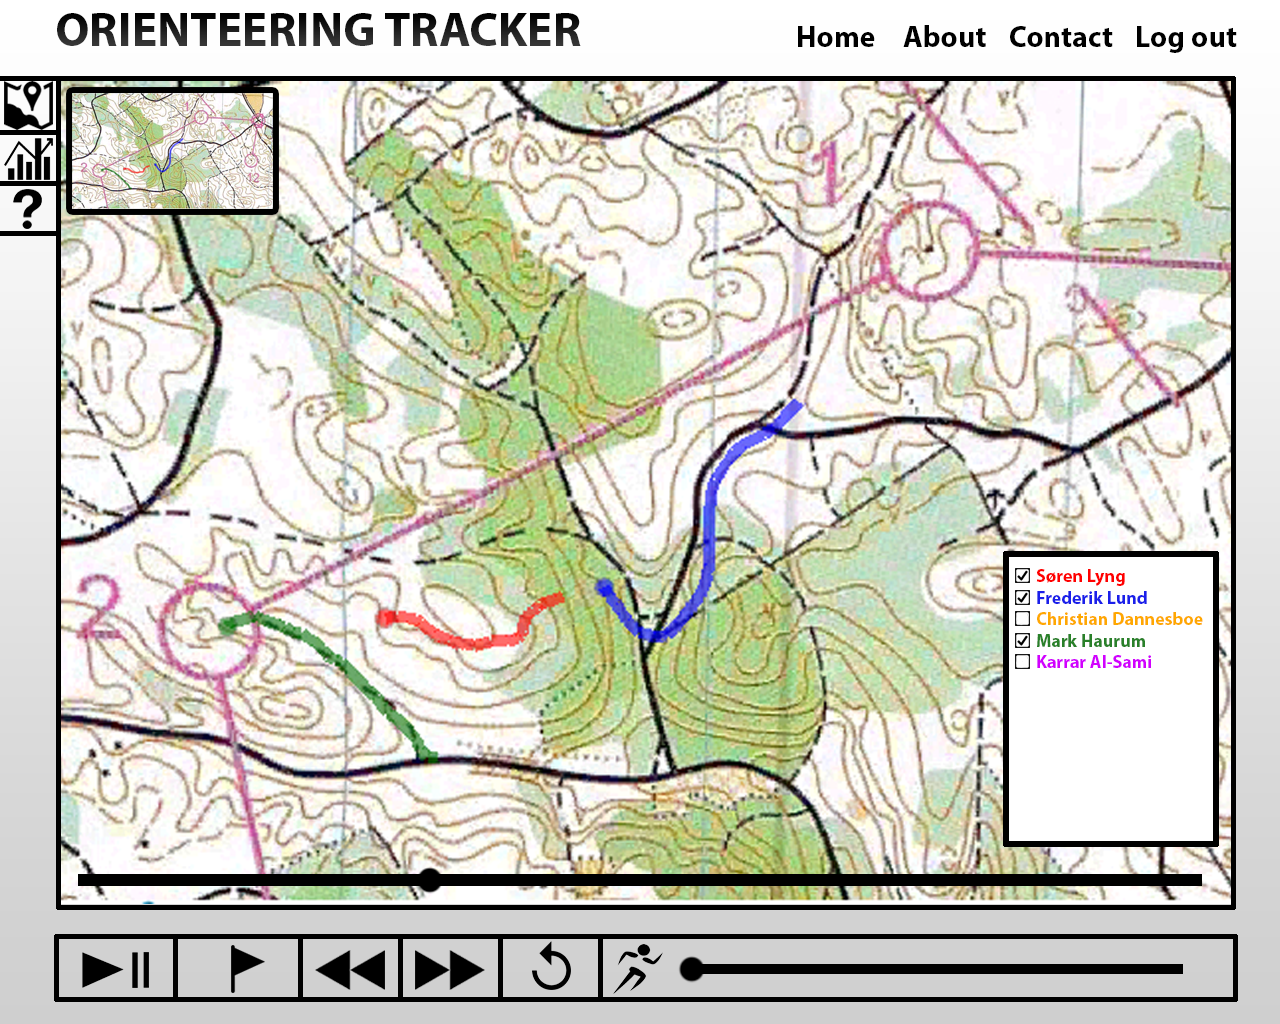
\includegraphics[width=1.0\textwidth]{billeder/Website_udkast_1}}
    \caption{Interface til webservice}
\end{figure}

\begin{figure}[h]
    \centering
    \fbox{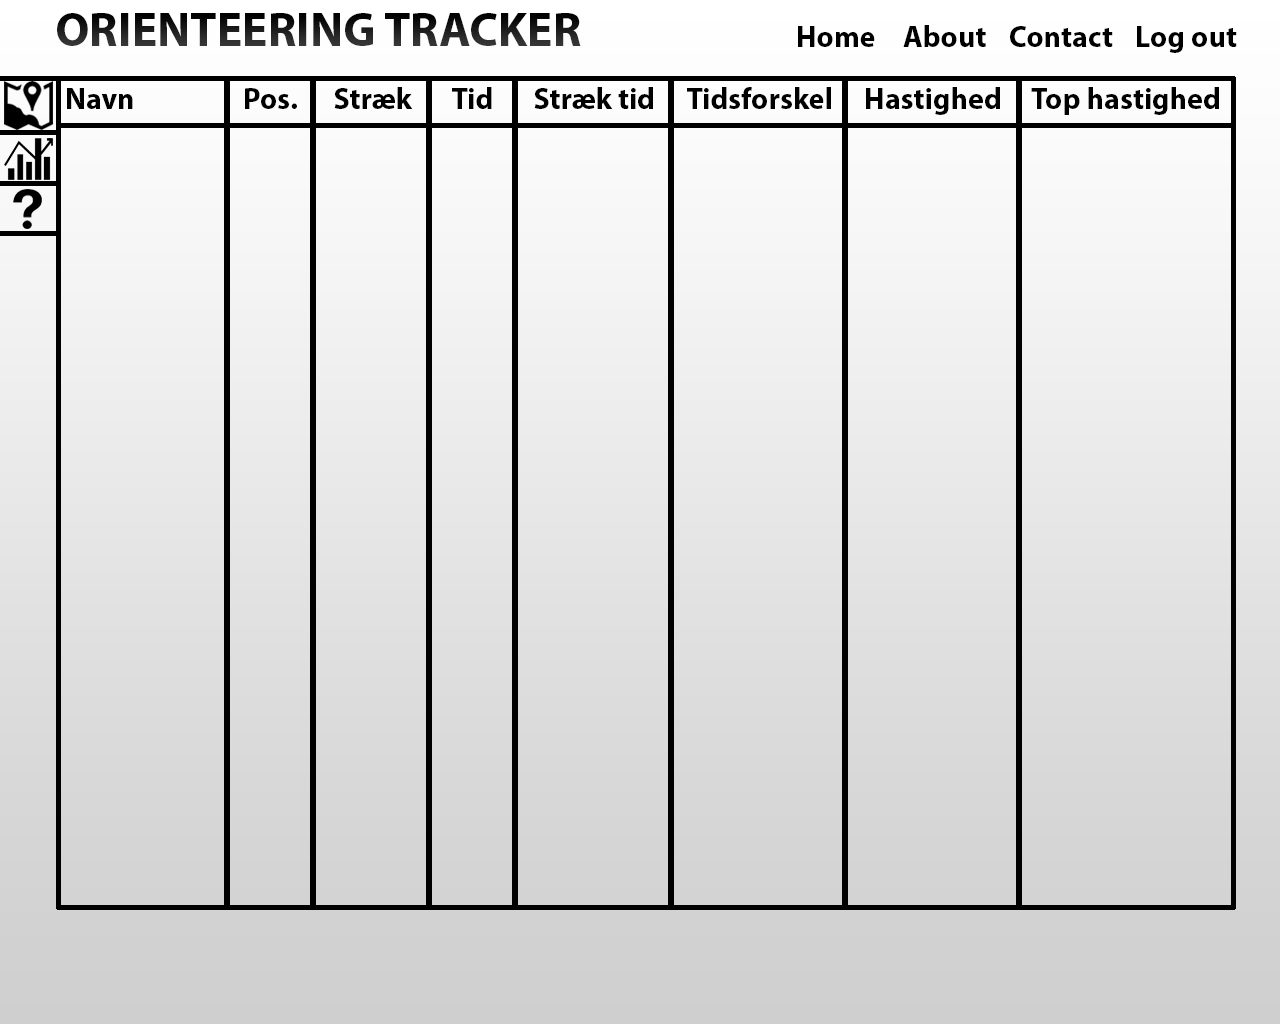
\includegraphics[width=1.0\textwidth]{billeder/Website_udkast_2}}
    \caption{Detaljeret sammenligning af løbere}
\end{figure}